\scanpage{56}
% E: display|upper left, pencil sum|nu_s1 minus one
\[
(\nu_{s_1}-1)+(\nu_{s_2}-1)\unsure{\cdots|+\cdots}
 +(\nu_{\unsure{s_n|s_0}}-1)
\]
\inserted{\(\unsure{\nu_{s_0}}\)}

% E: drawing|upper left|circle with three attached polygons arrows zero one
\figure{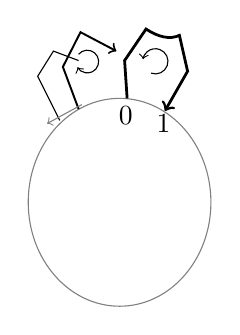
\begin{tikzpicture}[scale=.8]
\draw[gray] (0,0) ellipse(1.45 and 1.65);
\draw (-.95,1.3)--(-1.3,2)--(-1.05,2.4)--(-.65,2.25);
\draw[line width=.7pt,->] (-.65,1.48)--(-.9,2.15)--(-.62,2.7)--(-.05,2.4);
\draw[line width=1pt,->] (.12,1.65)--(.08,2.25)--(.42,2.75)..controls (.62,2.62) and (.8,2.58)..(.95,2.65)--(1.08,2.08)--(.72,1.45);
\draw[->] (-.65,2.35) arc(140:-150:.18); \draw[->] (.5,2.05) arc(-110:170:.2);
\draw[gray,->] (-.6,1.55)--(-1.15,1.25);
\node at (.1,1.37) {$0$}; \node at (.7,1.25) {$1$};
\end{tikzpicture}}

% E: drawing|upper centre-left|vertical interval with s1 s0 s n-1
\figure{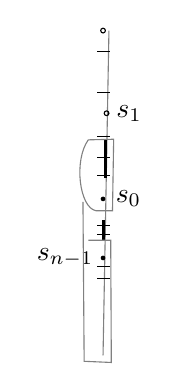
\begin{tikzpicture}[scale=.75]
\draw[gray] (0,0)--(.1,5.5);
\draw (0,5.5) circle(.04) (.06,4.1) circle(.04);
\foreach \y in {1.3,1.5,2.05,2.2,3.05,3.35,3.7,4.45,5.15}{\draw (-.1,\y)--(.12,\y);}
\fill (0,2.65) circle(.04) (0,1.65) circle(.04);
\node[right] at (.06,4.1) {$s_1$}; \node[right] at (.05,2.65) {$s_0$}; \node[left] at (0,1.65) {$s_{n-1}$};
\draw[line width=1.1pt] (.04,3)--(.04,3.65) (0,1.95)--(0,2.3);
\draw[gray] (-.25,3.65)..controls (-.5,3.3) and (-.4,2.5)..(-.12,2.45)--(.16,2.45)--(.18,3.66)--cycle;
\draw[gray] (-.34,2.6)--(-.32,-.1)--(.14,-.12)--(.13,1.95)--(-.25,1.95);
\end{tikzpicture}}

% E: display|left middle, lengths|l_s equals n minus nu_s
\[
\begin{aligned}
\ell_s&=\deleted{\unsure{\ell_0}}n-\nu_s\\
\ell_a&=\deleted{\unsure{\ell}}n-1-(\nu_s-1)-(\nu_t-1)\\
&=n\deleted{\unsure{+}}\inserted{-}(\nu_s+\nu_t-1)=(n-\nu_s)-(\nu_t-1)\\
\ell_s-\ell_a&=\nu_t-1\qquad \unsure{=|\geq}\deleted{\unsure{\nu_t}}\unsure{1}
\end{aligned}
\]

% E: display|left middle-lower, sum|chi_2n sum multiplicities
\[
\chi_{2n}(\unsure{s|0})=\sum_{\substack{s\ \text{\unsure{tournant}}\\\text{sur }D_i}}(\nu(s)-1)=n-1
\qquad \mathbb Z/N\mathbb Z
\]
\inserted{multiplicité des sommets}

% E: display|left lower, lambda|lambda equals rho tilde
\[
\lambda(t)=\widetilde{\rho}_p(t)=(-1)^p(t-\chi_p)
\]
% E: text|left lower, parity|ici p equals 2n
ici \(p=2n\) donc \((-1)^p=+1\)

\deleted{\unsure{\(\rho\)}}\deleted{\(t\mapsto\)}
% E: display|left lower, simplified lambda|t minus chi_2n
\[
\lambda(t)=\deleted{\unsure{\ell}}t-\chi_{2n}=t-(n-1)
\]

% E: text|left bottom, NB|rho_p composition
\uline{NB}
\[
\begin{aligned}
\rho_p(t)&=\sigma_{p-1}\cdots\sigma_0(t)
=\deleted{(-1)^{p-1}(\chi_{\unsure{p|p-1}}-t)}\inserted{(-1)^p(t-\chi_p)}\\
&\deleted{=(-1)^p t+(-1)^{p-1}\chi_p}
\end{aligned}
\]

% E: text|bottom left, passage|Passage de F_p a F_0
Passage de \(F_p\) à \(F_0\) se fait par \(t\mapsto\deleted{\unsure{\ell_p-t}}t\)
\deleted{\unsure{(en effet, \(\ell_0=0\))}}

% E: drawing|central vertical face sequence|F p-1 F p F0 F1 F2 Fn Fn+1
\figure{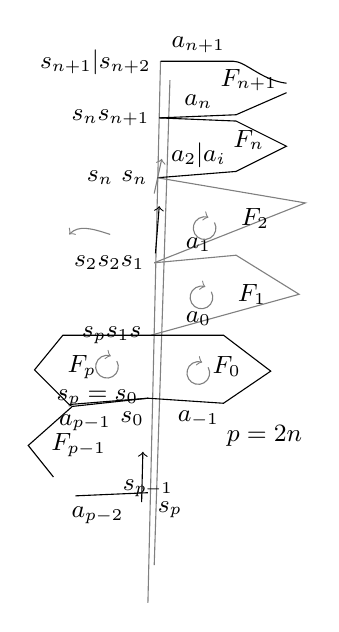
\begin{tikzpicture}[x=.8cm,y=.8cm,font=\small]
\draw[gray] (0,-1.4)--(.2,7.2);
\draw[gray] (.1,-.8)--(.35,6.9);
\draw[->] (-.1,.2)--(-.08,1); \draw[->] (.12,4.15)--(.18,4.9);
\draw[gray,->] (.1,5.1)--(.22,5.65);
\draw (.2,7.2)--(1.35,7.2)..controls (1.55,7.2) and (1.8,6.9)..(2.2,6.85);
\draw (2.2,6.7)--(1.4,6.35)--(.18,6.3);
\draw (.18,6.3)--(1.4,6.25)--(2.2,5.85)--(1.4,5.45)--(.15,5.35);
\draw[gray] (.15,5.35)--(2.5,4.95)--(.1,4);
\draw[gray] (.1,4)--(1.4,4.12)--(2.4,3.5)--(.05,2.85);
\draw (.05,2.85)--(1.2,2.85)--(1.95,2.28)--(1.2,1.77)--(0,1.85);
\draw (0,1.85)--(-1.25,1.75)--(-1.8,2.3)--(-1.35,2.85)--(.05,2.85);
\draw (0,1.85)--(-1.2,1.72)--(-1.9,1.1)--(-1.5,.6) (-1.15,.3)--(0,.35);
\node at (1.6,6.9) {$F_{n+1}$}; \node at (1.6,5.95) {$F_n$}; \node at (1.7,4.7) {$F_2$}; \node at (1.65,3.5) {$F_1$}; \node at (1.25,2.35) {$F_0$};
\node at (-1.05,2.35) {$F_p$}; \node at (-1.1,1.1) {$F_{p-1}$};
\node[above] at (.8,7.18) {$a_{n+1}$}; \node[left] at (.2,7.18) {$\unsure{s_{n+1}|s_{n+2}}$};
\node[above] at (.8,6.3) {$a_n$}; \node[left] at (.18,6.3) {$\deleted{\unsure{s_n}}s_{n+1}$};
\node[above] at (.8,5.35) {$\unsure{a_2|a_i}$}; \node[left] at (.15,5.35) {$s_n\ \unsure{s_n}$};
\node[above] at (.8,4.02) {$a_1$}; \node[left] at (.1,4) {$\deleted{\unsure{s_2}}s_2\unsure{s_1}$};
\node[above] at (.8,2.85) {$a_0$}; \node[left] at (.05,2.85) {$\unsure{s_p}\deleted{\unsure{s_1}}s$};
\node[below] at (.8,1.8) {$a_{-1}$}; \node[left] at (0,1.85) {$s_p=s_0$};
\node at (-.25,1.52) {$\deleted{\unsure{s_0}}$};
\node[below] at (-1,1.75) {$a_{p-1}$}; \node[below] at (-.8,.28) {$a_{p-2}$};
\node at (0,.42) {$\unsure{s_{p-1}}$}; \node at (.35,.08) {$\deleted{\unsure{s_p}}$};
\node at (1.85,1.25) {$p=2n$};
\foreach \xx/\yy in {.8/2.25,.85/3.45,.9/4.55,-.65/2.35}{\draw[gray,->] (\xx,\yy) ++(30:.18) arc(30:-290:.18);}
\draw[gray,->] (-.6,4.45)..controls (-.9,4.55) and (-1.1,4.6)..(-1.25,4.45);
\end{tikzpicture}}

% E: drawing|lower centre, pencil circle|circle surrounded by curved petals
\figure{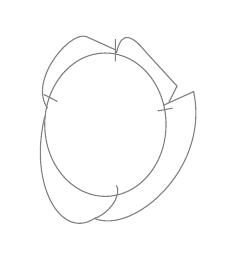
\begin{tikzpicture}[scale=.7]
\draw[gray] (0,0) ellipse (1.1 and 1.3);
\draw[gray] (-1.05,.3)..controls (-1.4,.8) and (-.65,1.7)..(-.35,1.6)--(.2,1.35);
\draw[gray] (.2,1.3)..controls (.3,1.75) and (.5,1.6)..(.75,1.3)--(1.3,.7)--(1.15,.4);
\draw[gray] (1.05,.35)--(1.6,.6)..controls (1.9,-.8) and (.5,-2)..(-.2,-1.7);
\draw[gray] (-1.1,.15)..controls (-1.4,-1.1) and (-.8,-2.1)..(-.2,-1.7)..controls (.1,-1.6) and (.3,-1.25)..(.2,-1.1);
\draw[gray] (-1.12,.55)--(-.87,.42) (.95,.25)--(1.22,.3) (.18,1.55)--(.18,1.15);
\end{tikzpicture}}

% E: diagram|right upper, element mapping|s n+1 maps to s n+1
\diagram{\begin{tikzcd}
s_{n+1}\arrow[r,mapsto] & s_{n+1}
\end{tikzcd}}

% E: diagram|right upper, square|P Fn to P Fn+1 and Z NZ
\diagram{\begin{tikzcd}
\unsure{P(F_n)|\operatorname{Pol}(F_n)}\arrow[r,"\sigma_{a_n}"] & \unsure{P(F_{n+1})|\operatorname{Pol}(F_{n+1})}\\
\mathbb Z/N\mathbb Z\arrow[u,no head,"\varphi_n","\wr"']\arrow[r,"\sigma_n"] & \deleted{\unsure{P}}\mathbb Z/N\mathbb Z\arrow[u,no head,"\varphi_{n+1}"',"\wr"]
\end{tikzcd}}

% E: text|right middle, properties|sigma_n respecte
\(\sigma_n\) respecte la structure polygonale

b) renverse l'orientation

c) transforme \(\underbrace{\varphi_n^{-1}(s_{n+1})}_{\ell_n}\) en \(\underbrace{\varphi_{n+1}^{-1}(s_{n+1})}_{0}\)

% E: display|right middle, conclusion|sigma_n t equals l_n minus t
donc \(\sigma_n(t)=\ell_n-t\)

% E: display|lower centre, three individual maps|sigma zero one n
\[
\begin{aligned}
\sigma_0(t)&=\ell_0-t\\
\sigma_1(t)&=\ell_1-t\\
\sigma_n(t)&=\ell_n-t
\end{aligned}
\]

% E: display|right lower, compositions|sigma1 sigma0
\[
\begin{aligned}
\sigma_1\sigma_0(t)&=\ell_1-(\ell_0-t)=\ell_1-\ell_0+t\\
\sigma_2\sigma_1\sigma_0(t)&=\ell_2-\ell_1+\ell_0-t\\
\underbrace{\overbrace{(\sigma_n\deleted{\unsure{\sigma}}\sigma_{n-1}\cdots\sigma_0)}^{n+1\ \text{facteurs}}}_{\rho_{n+1}}(t)
&=\ell_n-\ell_{n-1}\unsure{-\cdots|+\cdots}+(-1)^n\ell_0+(-1)^{n+1}t\\
&=(-1)^n(\chi_{n+1}-t)=(-1)^{n+1}(t-\chi_{n+1})
\end{aligned}
\]
% E: display|right bottom, alternating sum|chi n+1
où \(\displaystyle\chi_{n+1}=\underbrace{\ell_0\unsure{-|+}\ell_1\cdots+(-1)^n\ell_n}_{n+1\ \text{termes}}\)

% E: display|bottom edge, unfinished formula|sigma p-1 sigma p
\[
\underbrace{\sigma_{p-1}\sigma_{\unsure{p|p-2}}\cdots\sigma_0}_{\unsure{\rho_p}}(t)=(-1)^{p-1}
\]
\mspage{55}
